

\tikzset{every picture/.style={line width=0.75pt}} %set default line width to 0.75pt        

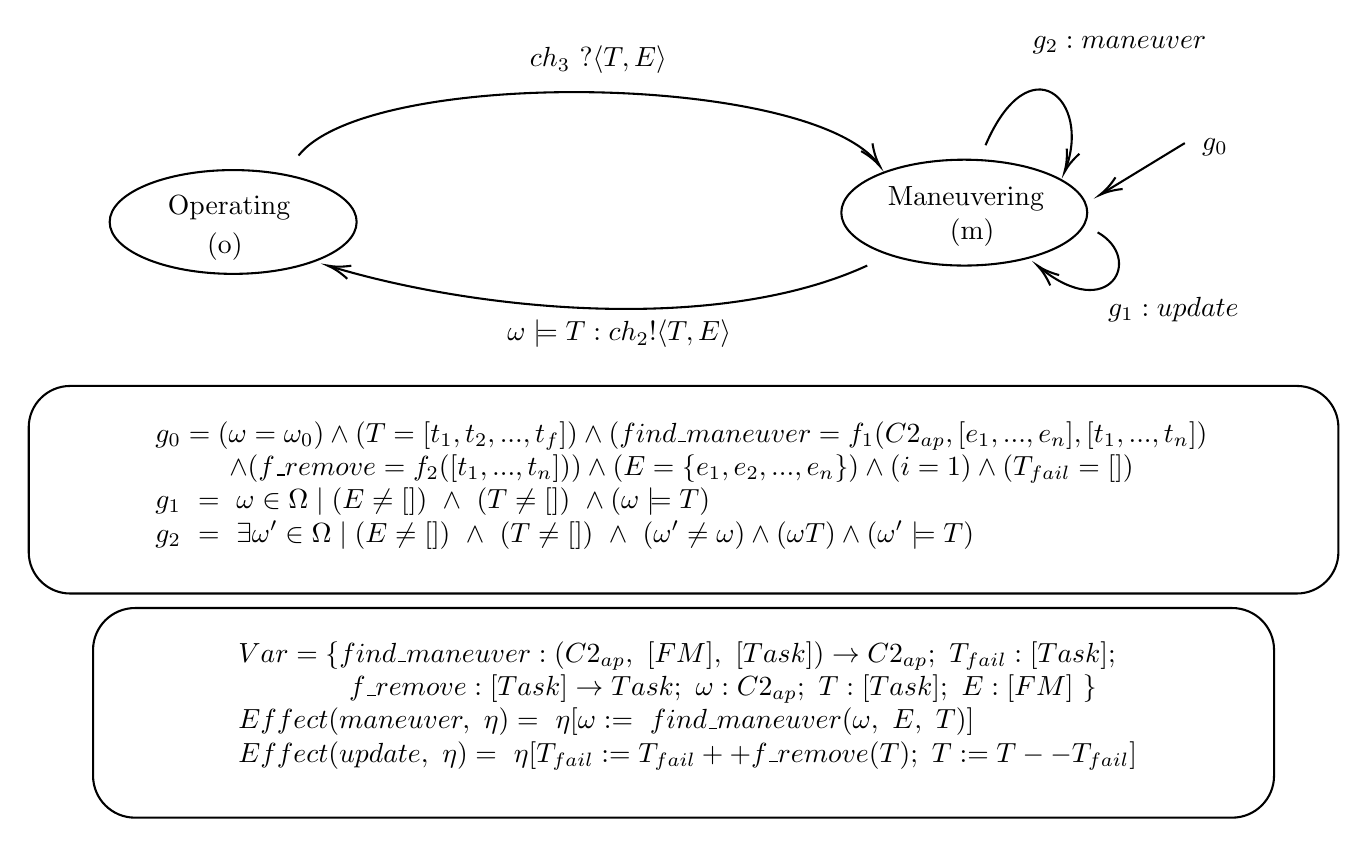
\begin{tikzpicture}[x=0.75pt,y=0.75pt,yscale=-1,xscale=1]
%uncomment if require: \path (0,397); %set diagram left start at 0, and has height of 397

%Curve Lines [id:da9480858267519683] 
\draw    (135.5,66) .. controls (169.16,23.43) and (380.22,25.94) .. (414.52,69.66) ;
\draw [shift={(415.5,71)}, rotate = 235.44] [color={rgb, 255:red, 0; green, 0; blue, 0 }  ][line width=0.75]    (10.93,-3.29) .. controls (6.95,-1.4) and (3.31,-0.3) .. (0,0) .. controls (3.31,0.3) and (6.95,1.4) .. (10.93,3.29)   ;
%Shape: Ellipse [id:dp6594609066072359] 
\draw   (44.5,98) .. controls (44.5,84.19) and (71.14,73) .. (104,73) .. controls (136.86,73) and (163.5,84.19) .. (163.5,98) .. controls (163.5,111.81) and (136.86,123) .. (104,123) .. controls (71.14,123) and (44.5,111.81) .. (44.5,98) -- cycle ;
%Shape: Ellipse [id:dp873836537729809] 
\draw   (397,93.5) .. controls (397,79.42) and (423.53,68) .. (456.25,68) .. controls (488.97,68) and (515.5,79.42) .. (515.5,93.5) .. controls (515.5,107.58) and (488.97,119) .. (456.25,119) .. controls (423.53,119) and (397,107.58) .. (397,93.5) -- cycle ;
%Curve Lines [id:da21020703050779688] 
\draw    (466.5,61) .. controls (487.68,11.75) and (517.59,39.15) .. (505.1,72.47) ;
\draw [shift={(504.5,74)}, rotate = 292.38] [color={rgb, 255:red, 0; green, 0; blue, 0 }  ][line width=0.75]    (10.93,-3.29) .. controls (6.95,-1.4) and (3.31,-0.3) .. (0,0) .. controls (3.31,0.3) and (6.95,1.4) .. (10.93,3.29)   ;
%Curve Lines [id:da14662580418826565] 
\draw    (520.5,103) .. controls (543.16,115.81) and (526.03,147.04) .. (493.02,120.26) ;
\draw [shift={(491.5,119)}, rotate = 400.46000000000004] [color={rgb, 255:red, 0; green, 0; blue, 0 }  ][line width=0.75]    (10.93,-3.29) .. controls (6.95,-1.4) and (3.31,-0.3) .. (0,0) .. controls (3.31,0.3) and (6.95,1.4) .. (10.93,3.29)   ;
%Straight Lines [id:da37650774099478246] 
\draw    (562.5,60) -- (523.21,83.96) ;
\draw [shift={(521.5,85)}, rotate = 328.63] [color={rgb, 255:red, 0; green, 0; blue, 0 }  ][line width=0.75]    (10.93,-3.29) .. controls (6.95,-1.4) and (3.31,-0.3) .. (0,0) .. controls (3.31,0.3) and (6.95,1.4) .. (10.93,3.29)   ;
%Rounded Rect [id:dp20897962983691354] 
\draw   (5.5,197) .. controls (5.5,185.95) and (14.45,177) .. (25.5,177) -- (616.5,177) .. controls (627.55,177) and (636.5,185.95) .. (636.5,197) -- (636.5,257) .. controls (636.5,268.05) and (627.55,277) .. (616.5,277) -- (25.5,277) .. controls (14.45,277) and (5.5,268.05) .. (5.5,257) -- cycle ;
%Rounded Rect [id:dp6489541210438411] 
\draw   (36.5,304.2) .. controls (36.5,293.04) and (45.54,284) .. (56.7,284) -- (585.3,284) .. controls (596.46,284) and (605.5,293.04) .. (605.5,304.2) -- (605.5,364.8) .. controls (605.5,375.96) and (596.46,385) .. (585.3,385) -- (56.7,385) .. controls (45.54,385) and (36.5,375.96) .. (36.5,364.8) -- cycle ;
%Curve Lines [id:da13961356622291943] 
\draw    (409.5,119) .. controls (335.87,152.83) and (218.68,140.13) .. (150.52,119.31) ;
\draw [shift={(149.5,119)}, rotate = 377.15999999999997] [color={rgb, 255:red, 0; green, 0; blue, 0 }  ][line width=0.75]    (10.93,-3.29) .. controls (6.95,-1.4) and (3.31,-0.3) .. (0,0) .. controls (3.31,0.3) and (6.95,1.4) .. (10.93,3.29)   ;

% Text Node
\draw (102,91) node   [align=left] {Operating};
% Text Node
\draw (457,87) node   [align=left] {Maneuvering};
% Text Node
\draw (280,20) node    {$ch_{3} \ ?\langle T,E\rangle $};
% Text Node
\draw (577,62) node    {$g_{0}$};
% Text Node
\draw (557,140) node    {$g_{1} :update$};
% Text Node
\draw (531,13) node    {$g_{2} :maneuver$};
% Text Node
\draw (320,225) node    {$ \begin{array}{l}
g_{0} =( \omega =\omega _{0}) \land ( T=[ t_{1} ,t_{2} ,...,t_{f}]) \land ( find\_maneuver=f_{1}( C2_{ap} ,[ e_{1} ,...,e_{n}] ,[ t_{1} ,...,t_{n}])\\
\ \ \ \ \ \ \ \ \land ( f\_remove=f_{2}([ t_{1} ,...,t_{n}])) \land ( E=\{e_{1} ,e_{2} ,...,e_{n}\}) \land ( i=1) \land ( T_{fail} =[])\\
g_{1} \ =\ \nexists \omega \in \Omega \mid ( E\neq []) \ \land \ ( T\neq []) \ \land ( \omega \models T) \ \\
g_{2} \ =\ \exists \omega '\in \Omega \mid ( E\neq []) \ \land \ ( T\neq []) \ \land \ ( \omega '\neq \omega ) \land ( \omega \nvDash T) \land ( \omega '\models T)
\end{array}$};
% Text Node
\draw (460,103) node   [align=left] {(m)};
% Text Node
\draw (100,110) node   [align=left] {(o)};
% Text Node
\draw (323,331) node    {$ \begin{array}{l}
Var=\{find\_maneuver:( C2_{ap} ,\ [ FM] ,\ [ Task])\rightarrow C2_{ap} ;\ T_{fail} :[ Task] ;\ \\
\ \ \ \ \ \ \ \ \ \ \ \ f\_remove:[ Task]\rightarrow Task;\ \omega :C2_{ap} ;\ T:[ Task] ;\ E:[ FM] \ \}\\
Effect( maneuver,\ \eta ) =\ \eta [ \omega :=\ find\_maneuver( \omega ,\ E,\ T)]\\
Effect( update,\ \eta ) =\ \eta [ T_{fail} :=T_{fail} ++f\_remove( T) ;\ T:=T--T_{fail}]
\end{array}$};
% Text Node
\draw (290,152) node    {$\omega \models T:ch_{2} !\langle T,E\rangle $};


\end{tikzpicture}